\documentclass[border=8pt]{standalone}
\usepackage{tikz}
\usetikzlibrary{arrows.meta, calc}

\begin{document}
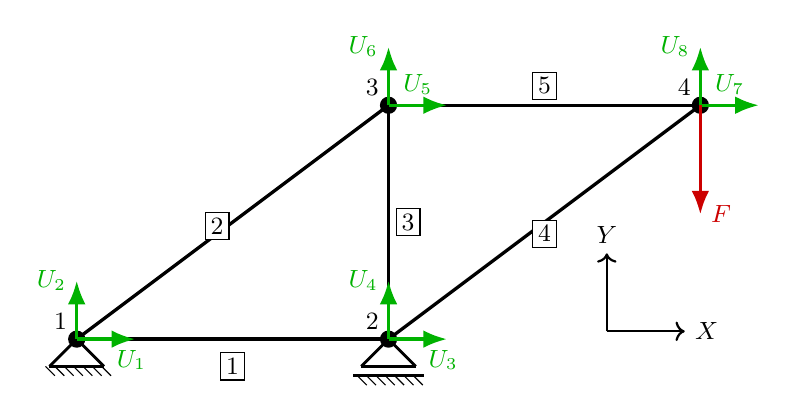
\begin{tikzpicture}[scale=0.99, every node/.style={font=\small},
    disp/.style={draw=green!70!black, very thick, -{Latex[length=3mm]}, green!70!black},
    load/.style={draw=red!80!black, very thick, -{Latex[length=3mm]}, red!80!black},
    member/.style={line width=1.2pt, black},
    joint/.style={circle, fill=black, inner sep=2.2pt},
    elbox/.style={draw, rectangle, inner sep=2pt, fill=white}
  ]
    % Knoten
    \coordinate (n1) at (0,0);
    \coordinate (n2) at (4,0);
    \coordinate (n3) at (4,3);
    \coordinate (n4) at (8,3);

    % Stäbe (Elemente)
    \draw[member] (n1) -- (n2); % e1
    \draw[member] (n1) -- (n3); % e2
    \draw[member] (n2) -- (n3); % e3
    \draw[member] (n2) -- (n4); % e4
    \draw[member] (n3) -- (n4); % e5

    % Gelenke
    \node[joint] at (n1) {};
    \node[joint] at (n2) {};
    \node[joint] at (n3) {};
    \node[joint] at (n4) {};

    % Knotennummern
    \node[above left] at (n1) {$1$};
    \node[above left] at (n2) {$2$};
    \node[above left] at (n3) {$3$};
    \node[above left] at (n4) {$4$};

    % Elementnummern
    \node[elbox] at (2.0,-0.35) {$1$};
    \node[elbox] at (1.8,1.45) {$2$};
    \node[elbox] at (4.25,1.5) {$3$};
    \node[elbox] at (6.0,1.35) {$4$};
    \node[elbox] at (6.0,3.25) {$5$};

    % Festlager Knoten 1 (Pin)
    \draw[line width=1pt] (n1) ++(-0.35,-0.35) -- ++(0.70,0);
    \draw[line width=1pt] (n1) ++(-0.35,-0.35) -- (n1);
    \draw[line width=1pt] (n1) ++(0.35,-0.35) -- (n1);
    \foreach \xx in {-0.40,-0.28,...,0.40} {\draw (n1) ++(\xx,-0.35) -- ++(0.12,-0.12);}

    % Loslager Knoten 2 (Roller, frei in x-Richtung)
    \draw[line width=1pt] (n2) ++(-0.35,-0.35) -- (n2);
    \draw[line width=1pt] (n2) ++(0.35,-0.35) -- (n2);
    \draw[line width=1pt] (n2) ++(-0.35,-0.35) -- ++(0.70,0);
    \draw[line width=1pt] (n2) ++(-0.45,-0.47) -- ++(0.90,0);
    \foreach \xx in {-0.40,-0.28,...,0.40} {\draw (n2) ++(\xx,-0.47) -- ++(0.12,-0.12);}

    % Verschiebungen (grün) + zugehörige Knotenkräfte (rot)
    \pgfmathsetmacro{\L}{0.75}

    % Knoten 1
    \draw[disp] (n1) -- ++(\L,0) node[midway, below right] {\color{green!70!black}$U_1$};
    \draw[disp] (n1) -- ++(0,\L) node[above, left] {\color{green!70!black}$U_2$};

    % Knoten 2
    \draw[disp] (n2) -- ++(\L,0) node[midway, below right] {\color{green!70!black}$U_3$};
    \draw[disp] (n2) -- ++(0,\L) node[above, left] {\color{green!70!black}$U_4$};

    % Knoten 3
    \draw[disp] (n3) -- ++(\L,0) node[midway, above] {\color{green!70!black}$U_5$};
    \draw[disp] (n3) -- ++(0,\L) node[above, left] {\color{green!70!black}$U_6$};

    % Knoten 4
    \draw[disp] (n4) -- ++(\L,0) node[midway, above] {\color{green!70!black}$U_7$};
    \draw[disp] (n4) -- ++(0,\L) node[above, left] {\color{green!70!black}$U_8$};

    % Last (rot)
    \draw[load] (n4) -- ++(0,-1.4) node[right] {$F$};

    % Koordinatensystem
    \draw[->,thick] (6.8,0.1) -- ++(1.0,0) node[right] {$X$};
    \draw[->,thick] (6.8,0.1) -- ++(0,1.0) node[above] {$Y$};
  \end{tikzpicture}
\end{document}
